\chapter{Vizualizace trasovacích dat}
\label{vizualizátory}

V této kapitole se zaměříme na to, proč je dobré mít vizualizátory dat a na nástroje sloužící k vizualizaci dat trasovacích. Jako vizualizátory bereme jakýkoliv typ software, který čte data a zobrazuje je přes nějaké grafické rozhraní. Mohou to být jednoduché skripty, které vytvoří soubory HTML a CSS pro zobrazení v internetovém prohlížeči, nebo samostatné aplikace s vlastními grafickými možnostmi.

\section{Proč vizualizovat}

Velmi rozšířeným typem systému je desktop. Počítač má dostatečné schopnosti na vytváření komplexnějších grafických aplikací. Toho spousta existujícího software využívá na zobrazení dat takovým způsobem, aby je lépe pochopili lidé. Ačkoliv rozhraní v terminálu je funkční a vhodné pro ostatní software, lidé více rozumí barvám, grafům a obrázkům, než pouhým seznamům a vypsaným číslům, hlavně pokud se jedná o mnoho dat. Terminál samotný má pak omezené schopnosti zobrazování grafiky, navíc ne všechny terminály jsou si rovny (např. terminály nemusí podporovat stejné barevné rozsahy). Trasovacích dat je mnoho, analyzovat v nich lze ledacos a (dobré) grafické rozhraní analýzu člověku usnadní, hlavně u dat o milionech událostí z velkých systémů.

Vizualizátory také mohou obsahovat funkcionality, které nejsou či nemohou být přítomny v nástrojích sloužících jako datový backend pro vizualizátory. Mohou to být například jednodušší rozhraní na vytváření filtrů či ukládání rozpracované analýzy, tj. například pozice v trasovacích datech a nějak vybrané události. Vizualizátory také mohou kombinovat data z více nástrojů, čímž se analýza zjednoduší, jelikož všechna potřebná data budou na jednom místě.

\section{HPerf}

HPerf \cite{Hperf-Pages} je frontendová aplikace pro nástroj Perf. Perf samotný se již snaží o pěkné zobrazení dat v terminálu, HPerf jde o krok dál a z dat vytvořených od \texttt{perf record} dokáže vytvořit stránku v HTML s JavaScriptem (viz obrázek \ref{hperfexample}), kterou lze navíc stylově upravovat pomocí vlastních CSS pravidel. HPerf dokáže vykonat práci \texttt{perf annotate} a \texttt{perf report} a navíc přidává vlastní funkcionality, to vše v GUI, k níž potřebujete pouze internetový prohlížeč s podporou JavaScriptu. Program má také minimální závislosti, jimiž jsou již zmíněný internetový prohlížeč, Perf, pak nástroje \texttt{objdump} a volitelně \texttt{highlight}. Na sestavení pak stačí použít buď GCC, nebo Clang, a program Make.

HPerf umí zobrazit assembly kód programu z dat a v okénku vedle i příslušnou část zdrojového kódu. Tato dvě okna jsou nezávislá. Okno se zdrojovým kódem navíc podporuje zvýrazňování syntaxe zkompilovaného jazyka.

HPerf dokáže pracovat s dlouhými trasovacími daty, ale velké binární soubory vytvoření HTML mohou zpomalit. Autor programu, Laurent Poirrier, toto vysvětluje nutností nahrát přes Objdump do paměti všechny assembly instrukce od všech dynamických sdílených objektů v trasovacích datech.

\begin{figure}[p]\centering
    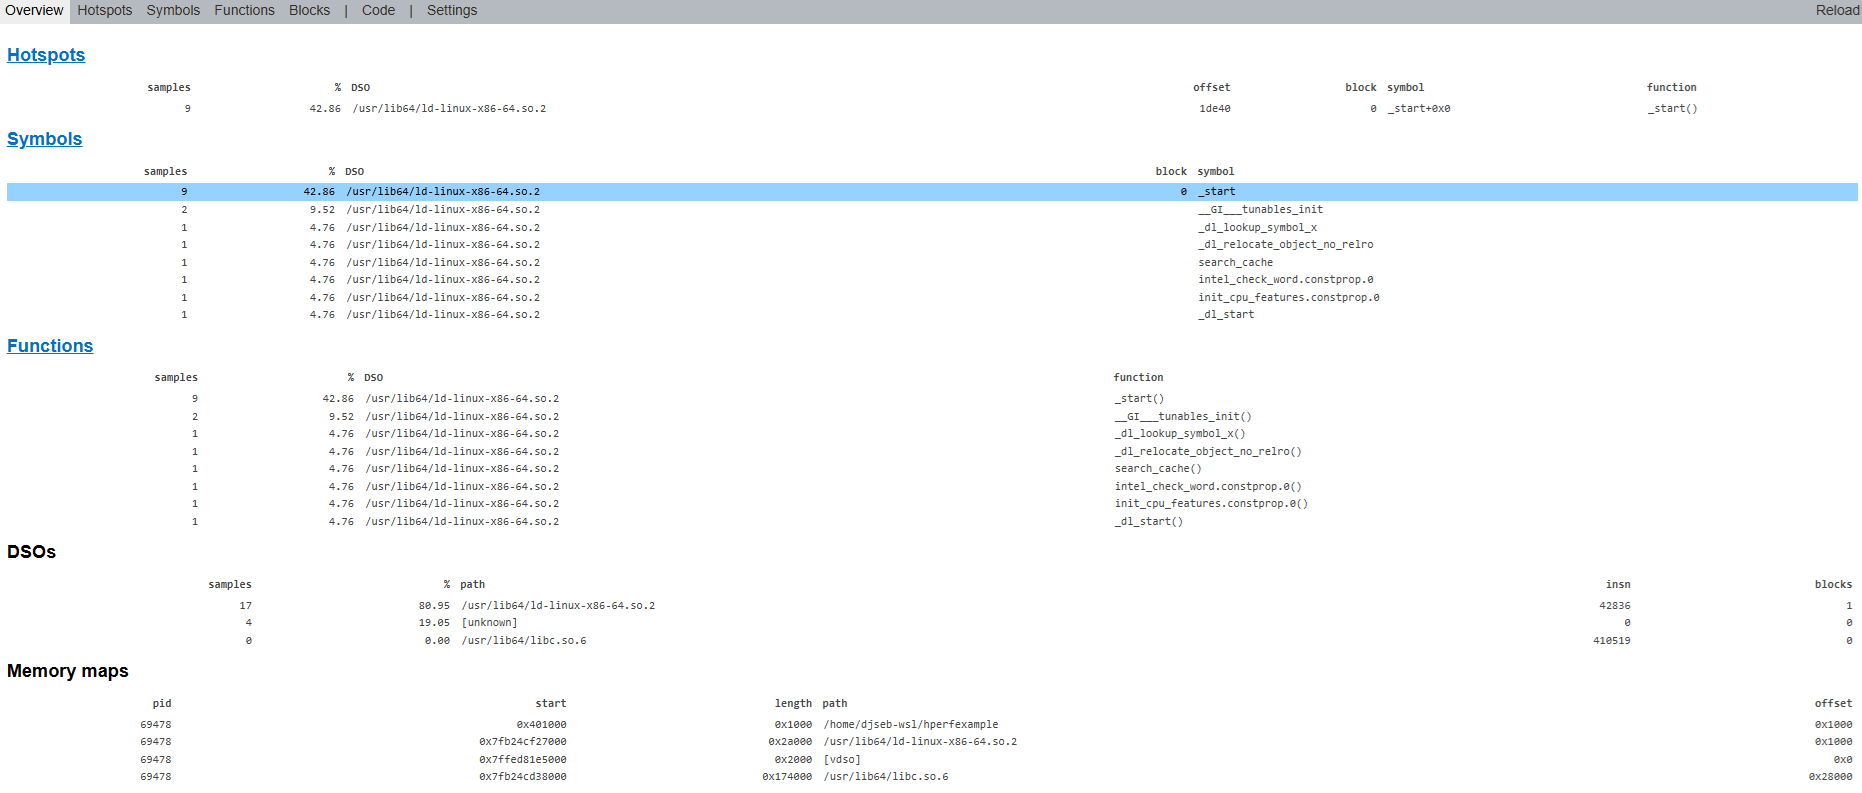
\includegraphics[width=140mm]{img/Vizualizátory/hperfexample.png}
    \caption{Ukázka GUI HPerf}
    \label{hperfexample}
\end{figure}

\section{Flame Graphs}
\label{flamegrafy}

Flame Graphs \cite{FlameGraphs-GitHub} jsou jedním z výtvorů Brendana Gregga, známé osobnosti ve vizualizaci trasovacích dat, momentálně zaměstnaným ve společnosti Intel. Flame Graphs jsou grafy, které zvýrazňují hierarchická data, primárně vytvořené pro zobrazení zásobníku systému. Nejníže jsou nejširší, tedy nejvíce časté, prvky z dat, které jsou abecedně seřazeny. Ve spodní vrstvě najdeme bloky odpovídající funkcím nejčastěji se vyskytujícím v nasbíraných datech. Čím širší blok, tím častěji se tato funkce na zásobníku objevuje. Nad každým blokem jsou pak \uv{potomci} (funkce volané z funkce v daném bloku). Tímto způsobem graf zobrazuje hierarchii volání.

Své jméno dostaly podle jejich tvaru a původnímu výběru barev, což byly hlavně teplé barvy. FlameGraph může vypadat například jako na obrázku \ref{bg-flamegraf} (příklad ze stránek Brendana Gregga \cite{FlameGraphs-Pages}). Tyto grafy se dají použít kromě zkoumání času na CPU i na průzkum času stráveném mimo CPU (např. když je proces blokován čekáním na data, nebo při preemptivním přepnutí), analýzu alokací paměti nebo celkem nově na vizualizaci profilování na GPU či AI akcelerátoru společně s celým zásobníkem, tzv. AI Flame Graphs. AI Flame Graphs mohou analyzovat výkonostní nedostatky běžící umělé inteligence a efektivně tak určit místa, kde by měly existovat optimalizace. Tím se může výrazně zlepšit spotřeba energie, pro kterou jsou umělé inteligence nechvalně známy.

\begin{figure}[p]\centering
    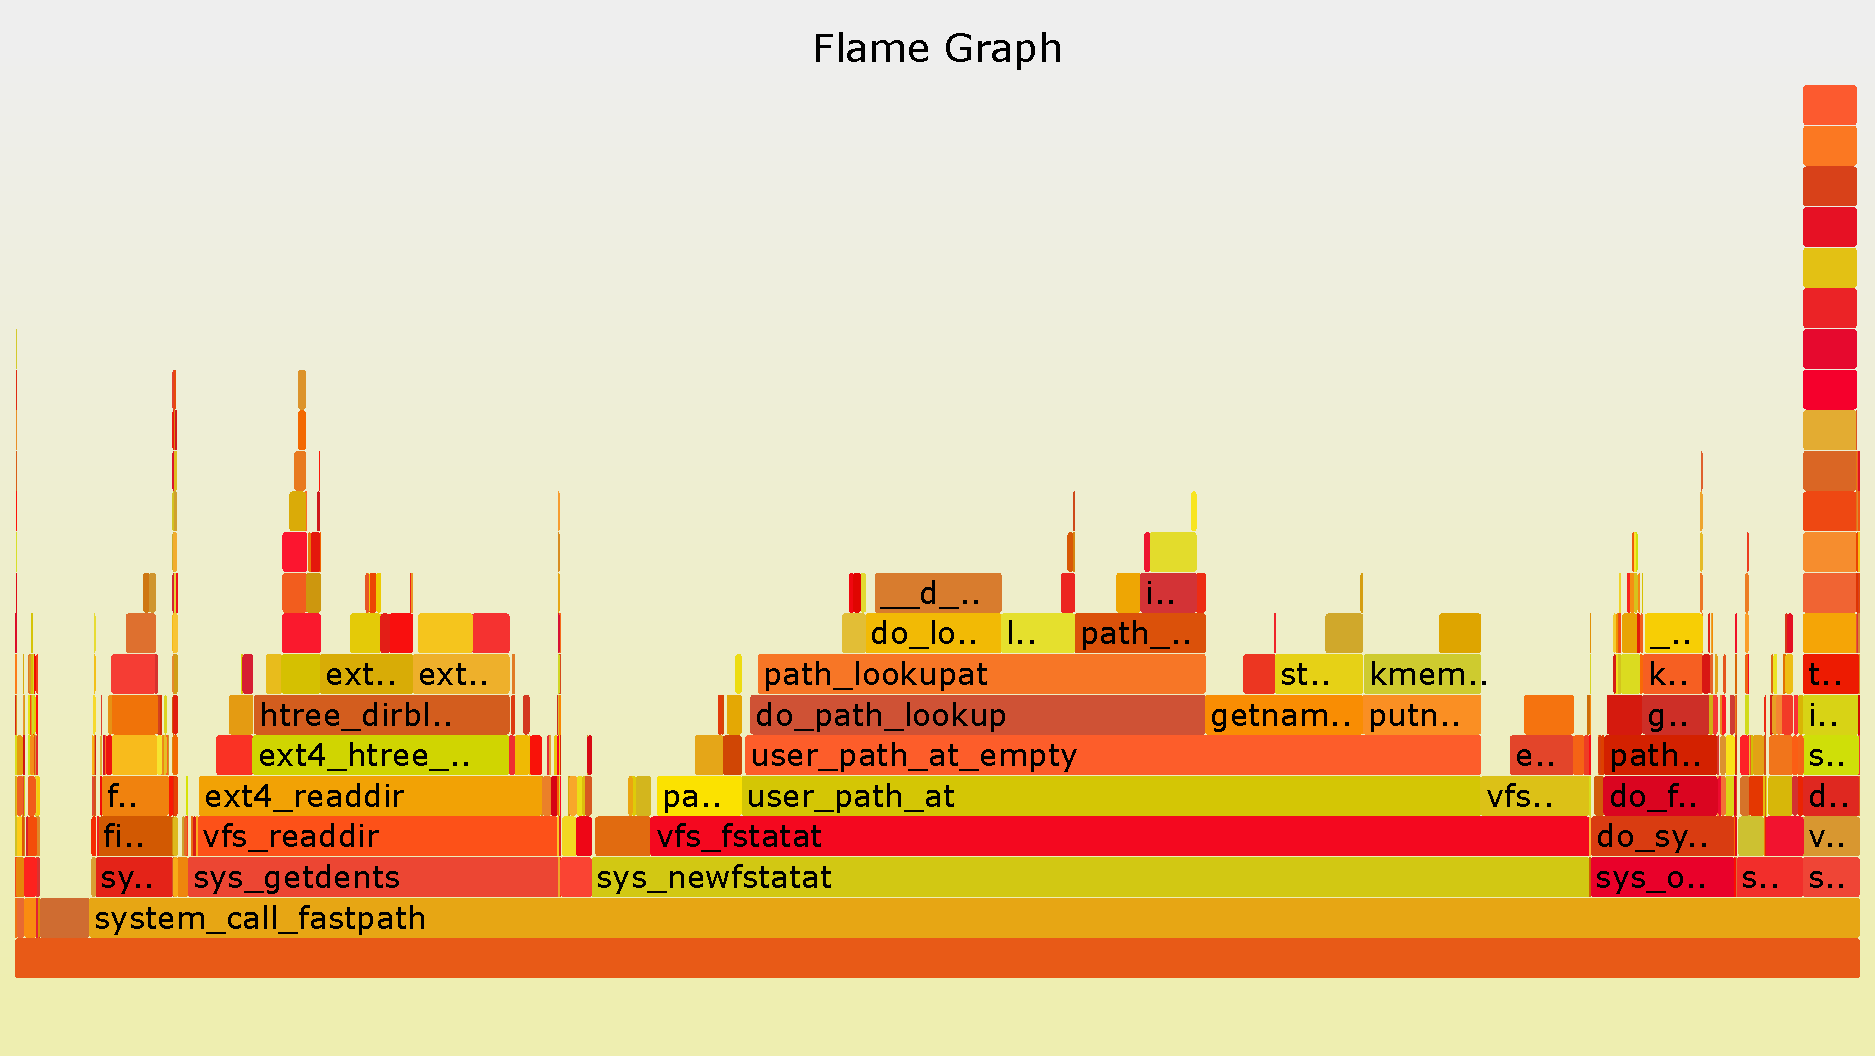
\includegraphics[width=140mm]{img/Vizualizátory/brendan-gregg-example_cpu-linux-tar.pdf}
    \caption{FlameGraph pro čas na CPU procesu programu Tar}
    \label{bg-flamegraf}
\end{figure}

Tato vizualizace je velmi rozšířena a existuje mnoho implementací. Některé mění barvy prvků tak, aby se ukázala příslušnost v kódu, některé vytváří \uv{rampouchové grafy}, tj. FlameGraph otočený vzhůru nohama, s chladnými barvami. Tento typ vizualizace se pak hodí, pokud jsou zásobníky dlouhé a vrchní oblast by byla příliš řídká. Zajímavou změnou jsou \uv{sunburst grafy}, kdy se FlameGraph transformuje do koláčového grafu, jak ukazuje obrázek \ref{sunburstgraf}, získaný z GitHubu tohoto projektu \cite{SunburstGraphs}.

\begin{figure}[p]\centering
    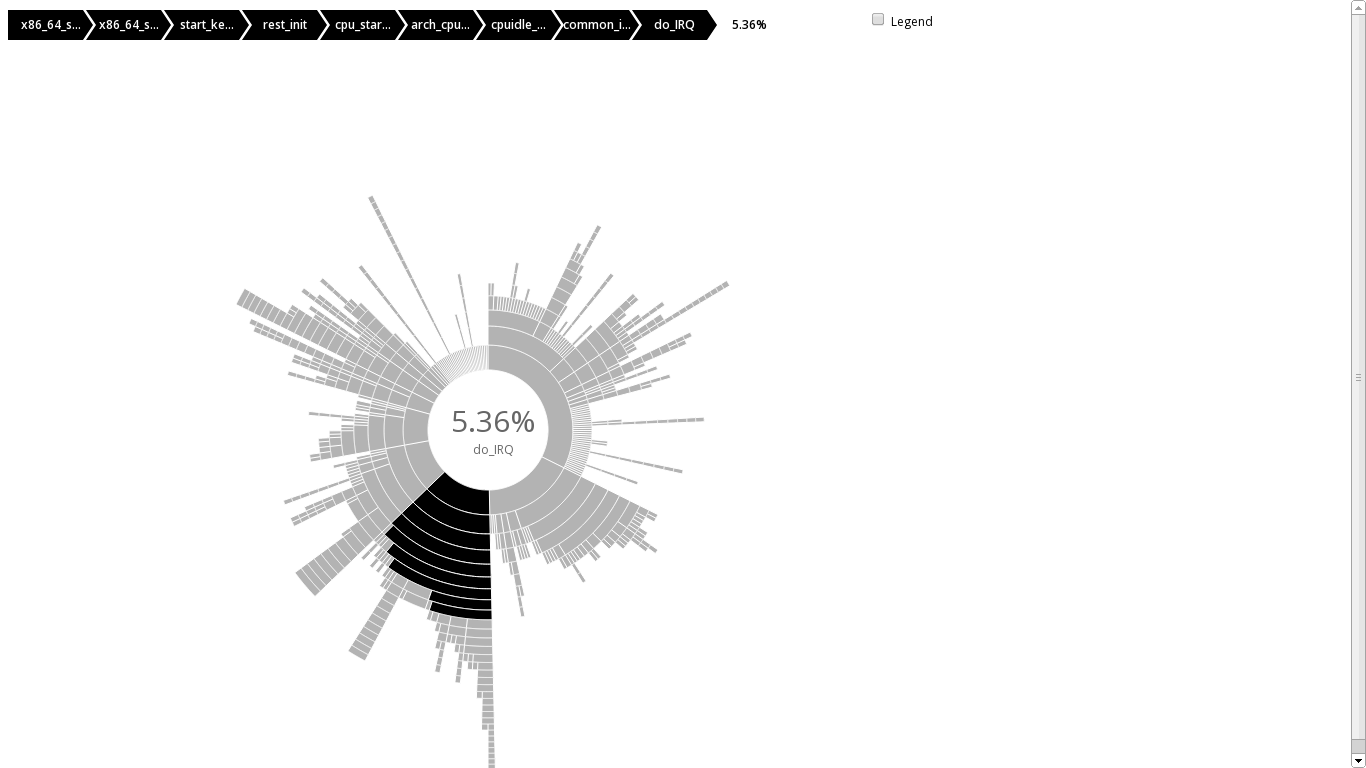
\includegraphics[width=140mm]{img/Vizualizátory/sunburstgraf.png}
    \caption{Ukázka sunburst grafu v akci}
    \label{sunburstgraf}
\end{figure}

Brendan Gregg nabízí i Perl program na vytváření FlameGraphů z dat Perfu nebo DTrace (trasovací nástroj od Sun Microsystems, původně pro operační systém Solaris, dnes podporuje více operačních systémů, včetně Linuxu a Windows), ale i mnoha dalších profilovacích nástrojů, pokud jsou schopny zásobník zachytit. Program extrahuje pouze data zajímavá pro něj a poté vytvoří vizualizaci. Pro tento nástroj existuje i několik možností chování, jako například vytvoření rampouchových grafů, či změna různých vlastností v SVG, jako například velikost písma, název grafu, použité barvy, nebo i přidání poznámek. Program je open-source a dostupný na GitHubu Brendana Gregga.

\section{TraceShark}

Prvním \uv{žraločím} nástrojem který si představíme je je TraceShark \cite{TraceShark}. Tento vizualizátor se zaměřuje na vizualizaci událostí plánovače úloh v kernelu, specificky na události přepínání kontextu, probuzení procesu, vytváření a zavírání procesů, frekvenci CPU a neaktivitu CPU. Tyto události musí být sesbírány buď přes Perf nebo Ftrace (či frontendy pro Ftrace, jako Trace-cmd). Nástroj je open-source a stále ve fázi vývoje, seznam podporovaných událostí tedy může dále růst. Ukázku GUI lze vidět na obrázku \ref{traceshark-github}, který je veřejně dostupný na GitHubu projektu. Mezi KernelSharkem a TraceSharkem neexistuje přímá spojitost, nicméně sdílí podobné rozhraní, některé cíle a podobné jméno.

\begin{figure}[p]\centering
    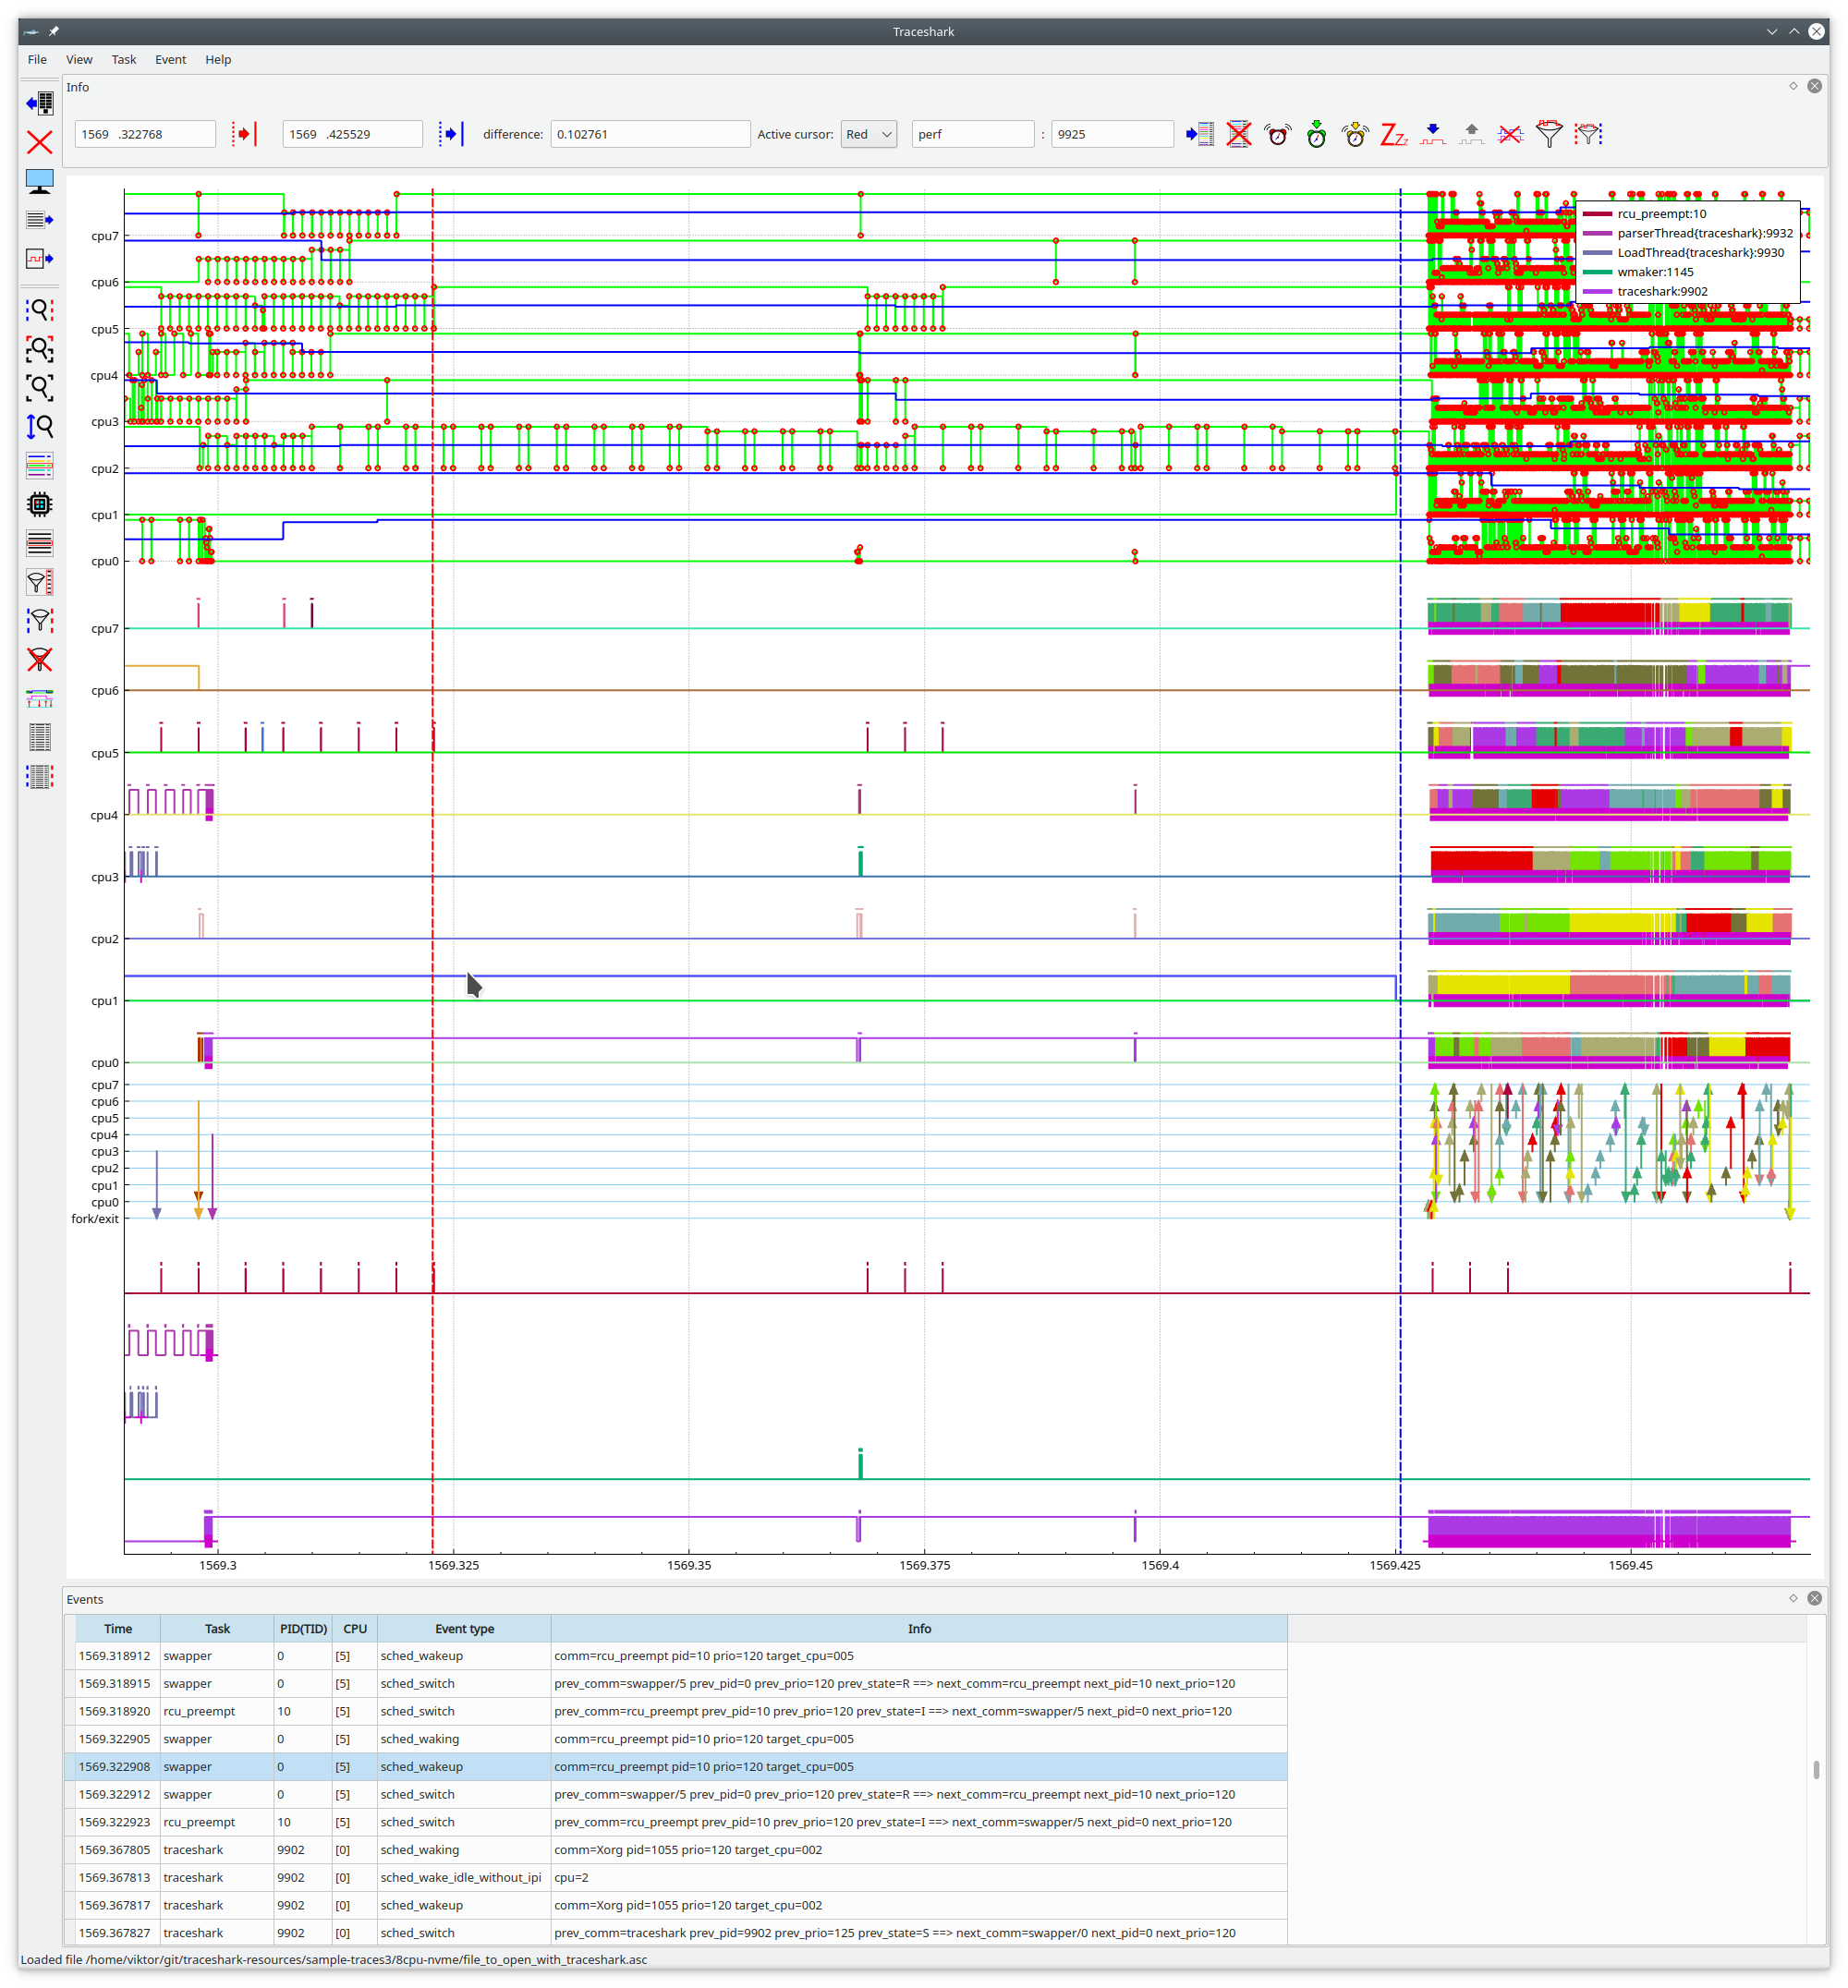
\includegraphics[width=140mm]{img/Vizualizátory/traceshark-git-hub-example.png}
    \caption{Ukázka GUI TraceSharku}
    \label{traceshark-github}
\end{figure}

TraceShark v první grafové sekci ukazuje aktivity na každém z detekovaných CPU a jejich frekvence. V další sekci na CPU grafech ukazuje pro každý procesor, které procesy na něm běžely a to pomocí různobarevných obdélníčků. Zde se zobrazují i latence mezi označením procesu za připravený ke spuštění a opravdovým přepnutím procesoru na kontext tohoto procesu. Každá z použitých barev vyjadřuje jednu úlohu. Třetí sekce s CPU grafy pak ukazuje migrace úloh mezi procesory pomocí různobarevných šipek. Poslední sekce je vyhrazena pro grafy jednotlivých úloh, které si může uživatel sám přidat přes GUI. V grafech se dá pohybovat vpravo a vlevo rolováním kolečka myši, či, při zmáčknutí příslušného tlačítka, nahoru a dolů. Pod plochou pro grafy je i seznam událostí v trasovacích datech. Se seznamem lze interagovat, čímž se některé akce odrazí i v grafové ploše.

TraceShark dokáže pro události zobrazit jejich zásobník, filtrovat zobrazené informace podle identifikátoru vybrané události, nebo filtrovat podle PID procesu vlastnícího vybranou událost a nebo filtrovat podle CPU vybrané události. Program dokáže vytvářet snímky grafů, exportovat data ve formě vhodné pro vytváření FlameGraph vizualizací a lze i konfigurovat, které grafové sekce budou zobrazeny.

\section{KernelShark}

Tento nástroj, druhý ze \uv{žraločích} nástrojů, zde rozebírat nebudeme, má vlastní kapitolu \ref{kap-kernel-shark}. Nicméně jeho zmínka zde je nutná, jelikož je to další z více známých vizualizátorů, hlavně jako primární frontend pro Trace-cmd.